\section{Objektorientierte Analyse}\label{analyse}
Im Zuge des Kapitels Analyse wird der Prototyp und das verwendete SAP UI5 Framework analysiert und die Ergebnisse in Form von Diagrammen gezeigt und beschrieben. Beginnend werden die Kombinationsmöglichkeiten zwischen den einzelnen Bibliotheken des SAP UI5 Frameworks aufgezeigt. Im Anschluss kommt eine Verdeutlichung eines Nachrichtenflusses innerhalb der SAP UI5 Applikation.

\subsection{Bibliotheken Beziehungen}
// Lib Diagramm beschreiben
Lorem ipsum dolor sit amet, consetetur sadipscing elitr, sed diam nonumy eirmod tempor invidunt ut labore et dolore magna aliquyam erat, sed diam voluptua. At vero eos et accusam et justo duo dolores et ea rebum. Stet clita kasd gubergren, no sea takimata sanctus est Lorem ipsum dolor sit amet. Lorem ipsum dolor sit amet, consetetur sadipscing elitr, sed diam nonumy eirmod tempor invidunt ut labore et dolore magna aliquyam erat, sed diam voluptua. At vero eos et accusam et justo duo dolores et ea rebum. Stet clita kasd gubergren, no sea takimata sanctus est Lorem ipsum dolor sit amet. Lorem ipsum dolor sit amet, consetetur sadipscing elitr, sed diam nonumy eirmod tempor invidunt ut labore et dolore magna aliquyam erat, sed diam voluptua. At vero eos et accusam et justo duo dolores et ea rebum. Stet clita kasd gubergren, no sea takimata sanctus est Lorem ipsum dolor sit amet. 

\vspace{1em}
\begin{figure}[htb]
  \centering
  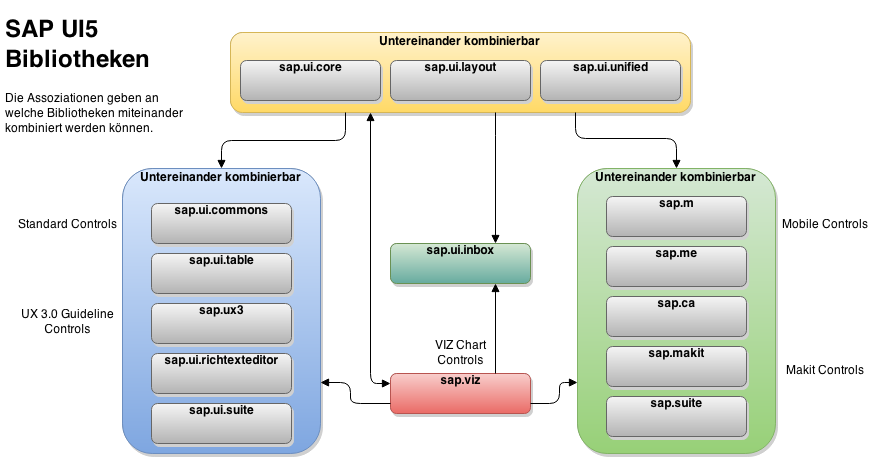
\includegraphics[width=1\linewidth]{abb/sapui5libconnections}
  \caption[Klassendiagramm: SAP UI5 Bibliotheken Kombinationen]{Klassendiagramm: SAP UI5 Bibliotheken Kombinationen}
  \label{fig:sapui5libconnections}
\end{figure}

\newpage
\subsection{Modularität}
// Paketdiagramm beschreiben und auf die Möglichkeiten des Templatings hinweisen. MVC Muster Stichwort
Lorem ipsum dolor sit amet, consetetur sadipscing elitr, sed diam nonumy eirmod tempor invidunt ut labore et dolore magna aliquyam erat, sed diam voluptua. At vero eos et accusam et justo duo dolores et ea rebum. Stet clita kasd gubergren, no sea takimata sanctus est Lorem ipsum dolor sit amet. Lorem ipsum dolor sit amet, consetetur sadipscing elitr, sed diam nonumy eirmod tempor invidunt ut labore et dolore magna aliquyam erat, sed diam voluptua. At vero eos et accusam et justo duo dolores et ea rebum. Stet clita kasd gubergren, no sea takimata sanctus est Lorem ipsum dolor sit amet. Lorem ipsum dolor sit amet, consetetur sadipscing elitr, sed diam nonumy eirmod tempor invidunt ut labore et dolore magna aliquyam erat, sed diam voluptua. At vero eos et accusam et justo duo dolores et ea rebum. Stet clita kasd gubergren, no sea takimata sanctus est Lorem ipsum dolor sit amet. 

\vspace{1em}
\begin{figure}[htb]
  \centering
  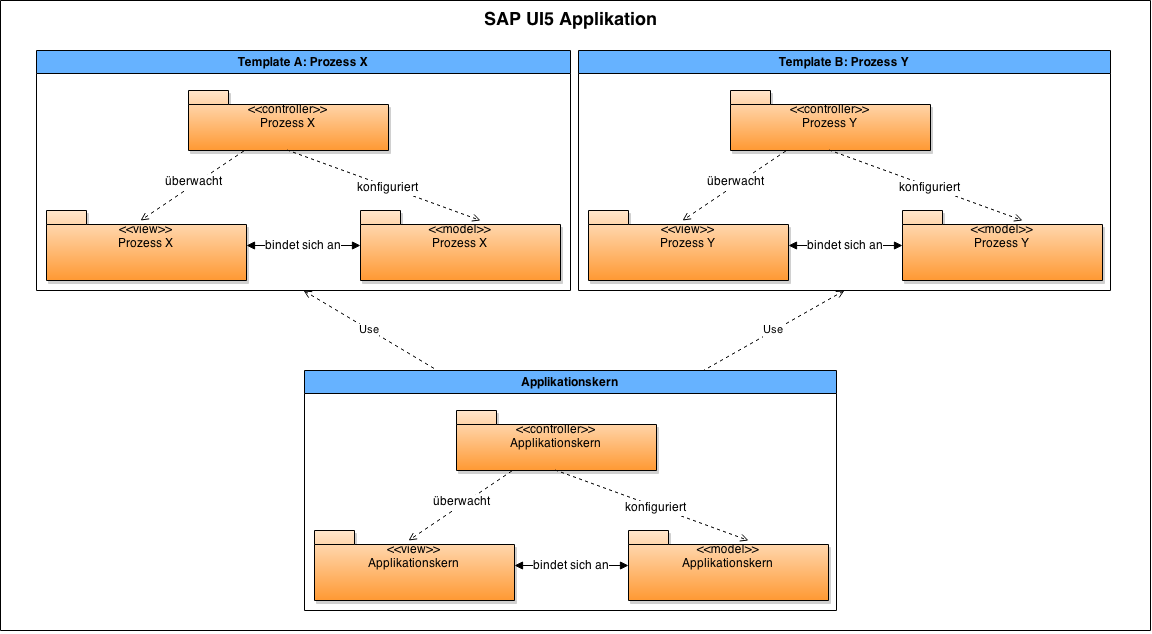
\includegraphics[width=1\linewidth]{abb/paketdiagramm}
  \caption[Paketdiagramm: MVC-Templates innerhalb einer SAP UI5 Applikation]{Paketdiagramm: MVC-Templates innerhalb einer SAP UI5 Applikation}
  \label{fig:paketdiagramm}
\end{figure}

\newpage
\subsection{UI Kaskade}
// Sequenzdiagramm beschreiben
Lorem ipsum dolor sit amet, consetetur sadipscing elitr, sed diam nonumy eirmod tempor invidunt ut labore et dolore magna aliquyam erat, sed diam voluptua. At vero eos et accusam et justo duo dolores et ea rebum. Stet clita kasd gubergren, no sea takimata sanctus est Lorem ipsum dolor sit amet. Lorem ipsum dolor sit amet, consetetur sadipscing elitr, sed diam nonumy eirmod tempor invidunt ut labore et dolore magna aliquyam erat, sed diam voluptua. At vero eos et accusam et justo duo dolores et ea rebum. Stet clita kasd gubergren, no sea takimata sanctus est Lorem ipsum dolor sit amet. Lorem ipsum dolor sit amet, consetetur sadipscing elitr, sed diam nonumy eirmod tempor invidunt ut labore et dolore magna aliquyam erat, sed diam voluptua. At vero eos et accusam et justo duo dolores et ea rebum. Stet clita kasd gubergren, no sea takimata sanctus est Lorem ipsum dolor sit amet. 

\vspace{1em}
\begin{figure}[htb]
  \centering
  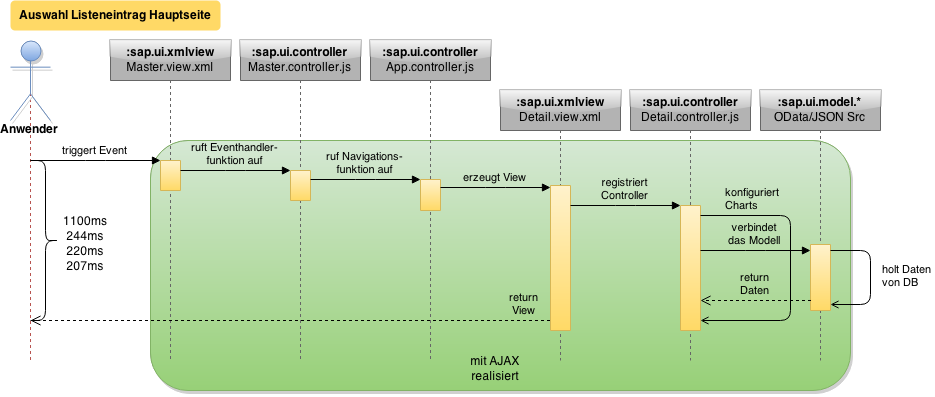
\includegraphics[width=0.95\linewidth,angle=90]{abb/sequence_load_list_entry}
  \caption[Sequenzdiagramm: Laden eines Listeneintrags]{Sequenzdiagramm: Laden eines Listeneintrags}
  \label{fig:sequenzdiagramm}
\end{figure}

\paragraph{Zeitmessung}$\;$ \\
// UI Zeitmessung kurz erklären wieso grade initial + 3 loads
// Tabelle \ref{tab:uiloading} zeigt
Lorem ipsum dolor sit amet, consetetur sadipscing elitr, sed diam nonumy eirmod tempor invidunt ut labore et dolore magna aliquyam erat, sed diam voluptua. At vero eos et accusam et justo duo dolores et ea rebum. Stet clita kasd gubergren, no sea takimata sanctus est Lorem ipsum dolor sit amet. Lorem ipsum dolor sit amet, consetetur sadipscing elitr, sed diam nonumy eirmod tempor invidunt ut labore et dolore magna aliquyam erat, sed diam voluptua. At vero eos et accusam et justo duo dolores et ea rebum. Stet clita kasd gubergren, no sea takimata sanctus est Lorem ipsum dolor sit amet. Lorem ipsum dolor sit amet, consetetur sadipscing elitr, sed diam nonumy eirmod tempor invidunt ut labore et dolore magna aliquyam erat, sed diam voluptua. At vero eos et accusam et justo duo dolores et ea rebum. Stet clita kasd gubergren, no sea takimata sanctus est Lorem ipsum dolor sit amet. 

\vspace{1em}
\begin{center}
  \begin{tabular}{ | c | c | c | c | c | }
    \hline
    \textbf{Versuch}
    & \textbf{Seite} & \textbf{1. Listeneintrag} & \textbf{2. Listeneintrag} & \textbf{3. Listeneintrag}\\
    \hline \hline
    1 & 1111ms & 230ms & 222ms & 205ms\\
    \hline
    2 & 1111ms & 230ms & 222ms & 205ms\\
    \hline
    3 & 1111ms & 230ms & 222ms & 205ms\\
    \hline
    4 & 1111ms & 230ms & 222ms & 205ms\\
    \hline
    5 & 1111ms & 230ms & 222ms & 205ms\\
    \hline
    6 & 1111ms & 230ms & 222ms & 205ms\\
    \hline
    7 & 1111ms & 230ms & 222ms & 205ms\\
    \hline
    8 & 1111ms & 230ms & 222ms & 205ms\\
    \hline
    9 & 1111ms & 230ms & 222ms & 205ms\\
    \hline
    10 & 1111ms & 230ms & 222ms & 205ms\\
    \hline \hline
    \O & 1111ms & 230ms & 222ms & 205ms\\
    \hline
  \end{tabular}
\captionof{table}{Chrome Browser UI Ladezeiten}
\label{tab:uiloading}
\end{center}

// Erkenntnis UI lädt ob cached oder uncached beim ersten Laden des UIs in nahezu unter 1,5 Sekunden. Jede weitere Auswahl eines Listeneintrags ist dann in durchschnittlich 233 Millisekunden fertig geladen und gerendert.
Lorem ipsum dolor sit amet, consetetur sadipscing elitr, sed diam nonumy eirmod tempor invidunt ut labore et dolore magna aliquyam erat, sed diam voluptua. At vero eos et accusam et justo duo dolores et ea rebum. Stet clita kasd gubergren, no sea takimata sanctus est Lorem ipsum dolor sit amet. Lorem ipsum dolor sit amet, consetetur sadipscing elitr, sed diam nonumy eirmod tempor invidunt ut labore et dolore magna aliquyam erat, sed diam voluptua. At vero eos et accusam et justo duo dolores et ea rebum.
